\chapter{Application}
\label{ch:Allpication}

The listed algorithms have their theoretical benefits, but we did not test them on real problems.  The numeric obstacles require the trade-offs between robustness, stability, and calculation time. The computer memory has limited capacity; systems discretization adds the plant errors. We considered the examples do not have a physical reference system. Now, we try to apply the algorithms on a more ''real'' plant and see the problems that occur. 

We consider a continuous-time 3-input 3-output system from \textit{COMPl$_{e^i}$b} \cite{CompLeib}, given as 
\begin{align}
\label{eq:Appl:realPlant} 
\begin{split}
\dot x(\tau) &= \begin{pmatrix}
0&         0&    1.132&         0&   -1\\
0&   -0.0538&   -0.1712&         0&    0.0705\\
0&         0&         0&    1&         0\\
0&    0.0485&         0&   -0.8556&   -1.013\\
0&   -0.2909&         0&    1.0532&   -0.6859\\
\end{pmatrix}x(\tau) + 
\begin{pmatrix}
0&         0&         0\\
-0.12&     1&         0\\
0&         0&         0\\
4.419&     0&   -1.6650\\
1.575&     0&   -0.0732
\end{pmatrix}u(\tau), \\
y(\tau) & = 
\begin{pmatrix}
1&     0&     0&     0&     0\\
0&     1&     0&     0&     0\\
0&     0&     1&     0&     0\\
\end{pmatrix}x(\tau), 
\end{split}
\end{align}
where $\tau$ is time in seconds, $0\leq \tau \leq 30$.

Since we are working with discrete time systems, we discretize it with Matlab command \comp{c2d}  for sample time \comp{Ts}$ = 10^{-3}$s  and get the state space description 
\begin{align}
\label{eq:Appl:discr_sys}
\left( \begin{array}{c | c}
A & B \\ \hline C & D
\end{array}\right) = 
\left(\begin{array}{c c c c c|c c c}
1&    0&    0.0011&    0&   -0.001&    0&    0&    0\\
0&    0.9999&   -0.0002&         0&    0.0001&   -0.0001&    0.001&   0\\
0&    0&    1&         0.001&   0&    0&    0&   0\\
0&    0&   0&         0.9991&   0&    0.0044&    0&   -0.0017\\
0&   -0.0003&    0&         0.0011&    0.9993&    0.0016&   0&   -0.0001\\\hline
1&    0&         0&         0&         0&         0&         0&         0\\
0&    1&         0&         0&         0&         0&         0&         0\\
0&         0&    1&         0&         0&         0&         0&         0
\end{array}\right). 
\end{align}
This discrete system is assumed to make $N$ steps, each with time increment of \comp{Ts}. 

\section{The case $D = 0$}

In the system \eqref{eq:Appl:discr_sys} the matrix $D$ is zero, what makes our algorithms not applicable. 
Moreover, the  $D$-part's neglecting is typical: the system output must mostly image the system state and not the known input we send.

But let us consider the output signal at discrete time increment $t\geq 1$:
\begin{align}
y(t) = C x(t) = CA x(t-1) + C B u(t-1).
\end{align}

Here the ''new'' $D$-term is represented by the matrix $CB$, if it is not zero. 
With other words, the input $u(\cdot)$ begins to impact the output after the first time step. We say, that the  \textit{relative degree} of the system equals 1. We define it mathematically precise.
\begin{defi}
	The relative degree of the system $(A, B, C, D)$ is 0 if $D \neq 0$. For $D = 0$ it is the smallest integer $k^*$ for which $	C A^{k^*-1} B \neq 0$.
\end{defi} 

We put the first $k^*$ terms away and consider our dynamical system from time step $k^*$:
\begin{align}
\begin{split}
x(t+1) &= A x(t) + B u(t), \\
y(t) &= C A^{k^* + 1}x(t) + C A^{k^*} B u(t),  \text{ for } t = k^*, k^* + 1, \dots N. 
\end{split}
\end{align}
The new initial condition equals $x(k^*)$, and the start input condition is $u(k^*)$. 

We can not approve the input signal at the first time steps, but still can improve it for the rest of them. 

\begin{exam}
For our system \eqref{eq:Appl:discr_sys} the relative degree is 1, as 
	\begin{align}
	CB = \begin{pmatrix}
	-7.8726e-07&	4.8474e-11&	3.656e-08\\
	-0.0001&	0.0009&		-2.5527e-09\\
	2.2086e-06&	8.0937-12&	-8.3225e-07\\
	\end{pmatrix}
	\end{align}
%TODO: Zahlen? 

The small values of the matrix elements result from the small terms of the matrix $B$, and in this case does not disturb us.

We calculate the solution with LQR. Result for each of the three dimentions is illustrated in Figure \ref{img:Appl:AC1_LQR}. 
\begin{figure}[H]
	\centering
	\begin{subfigure}[b]{0.3\textwidth}
		\centering
		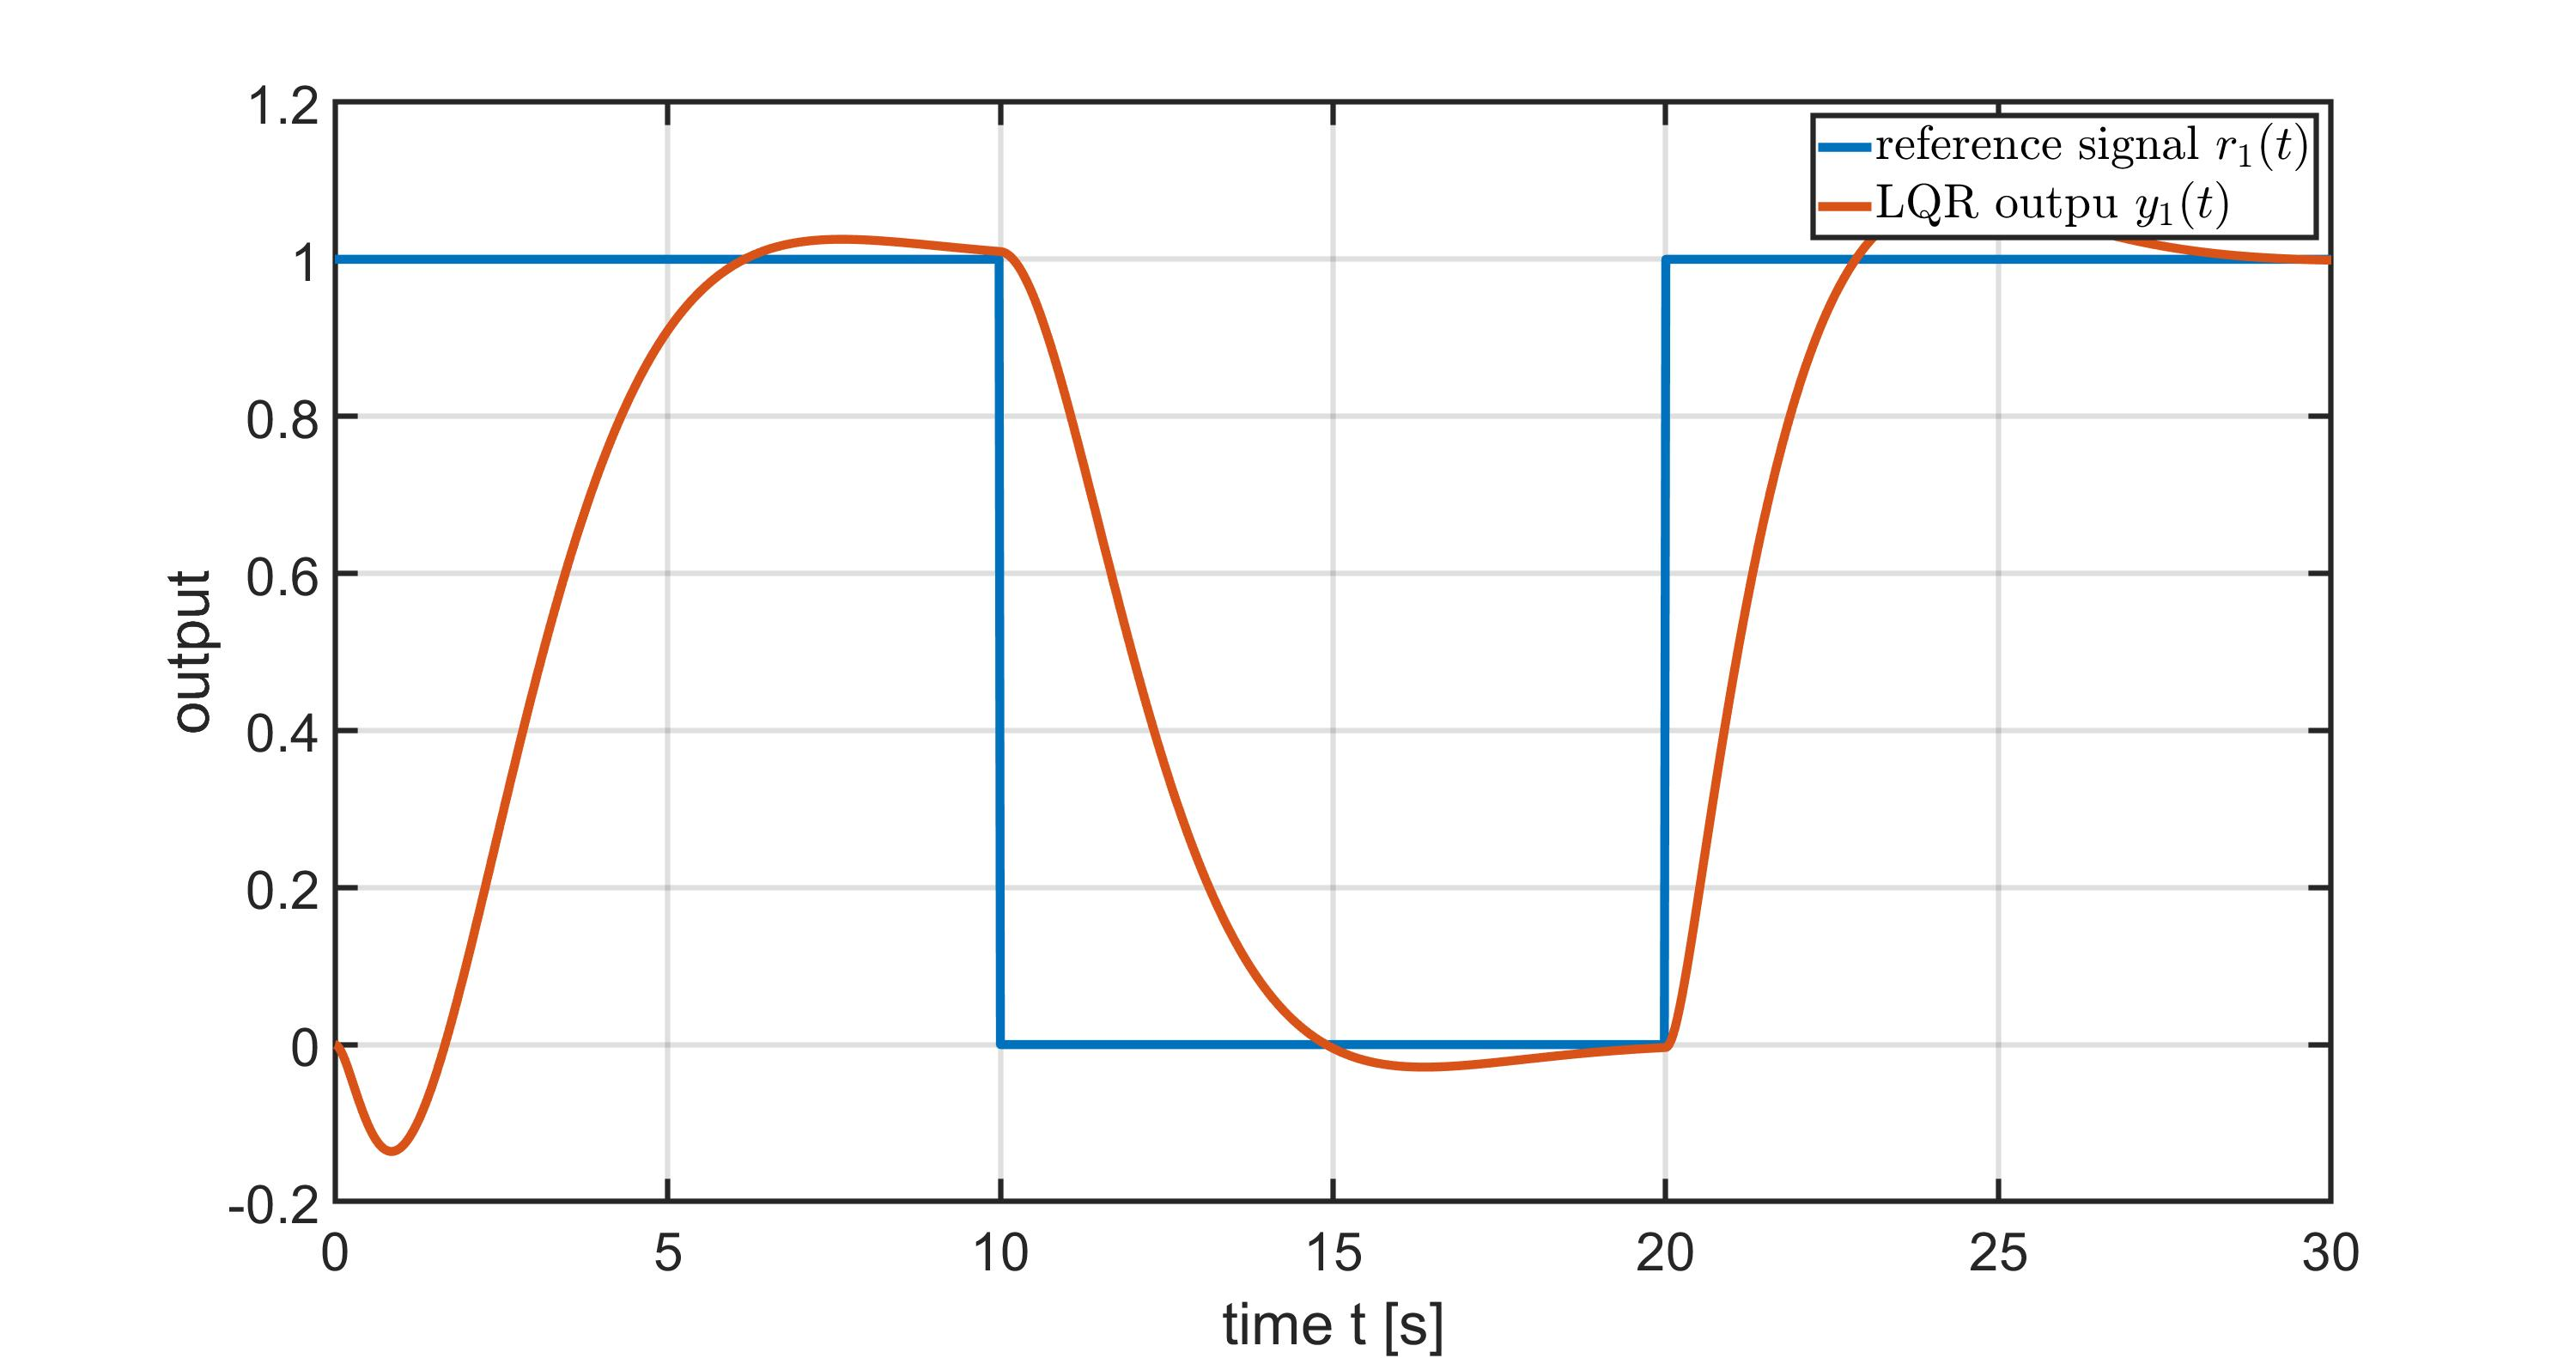
\includegraphics[width=\textwidth]{fig/AC1_LQR_1.jpg}
		\caption{First signal}
	\end{subfigure}
	\hfill
	\begin{subfigure}[b]{0.3\textwidth}
		\centering
		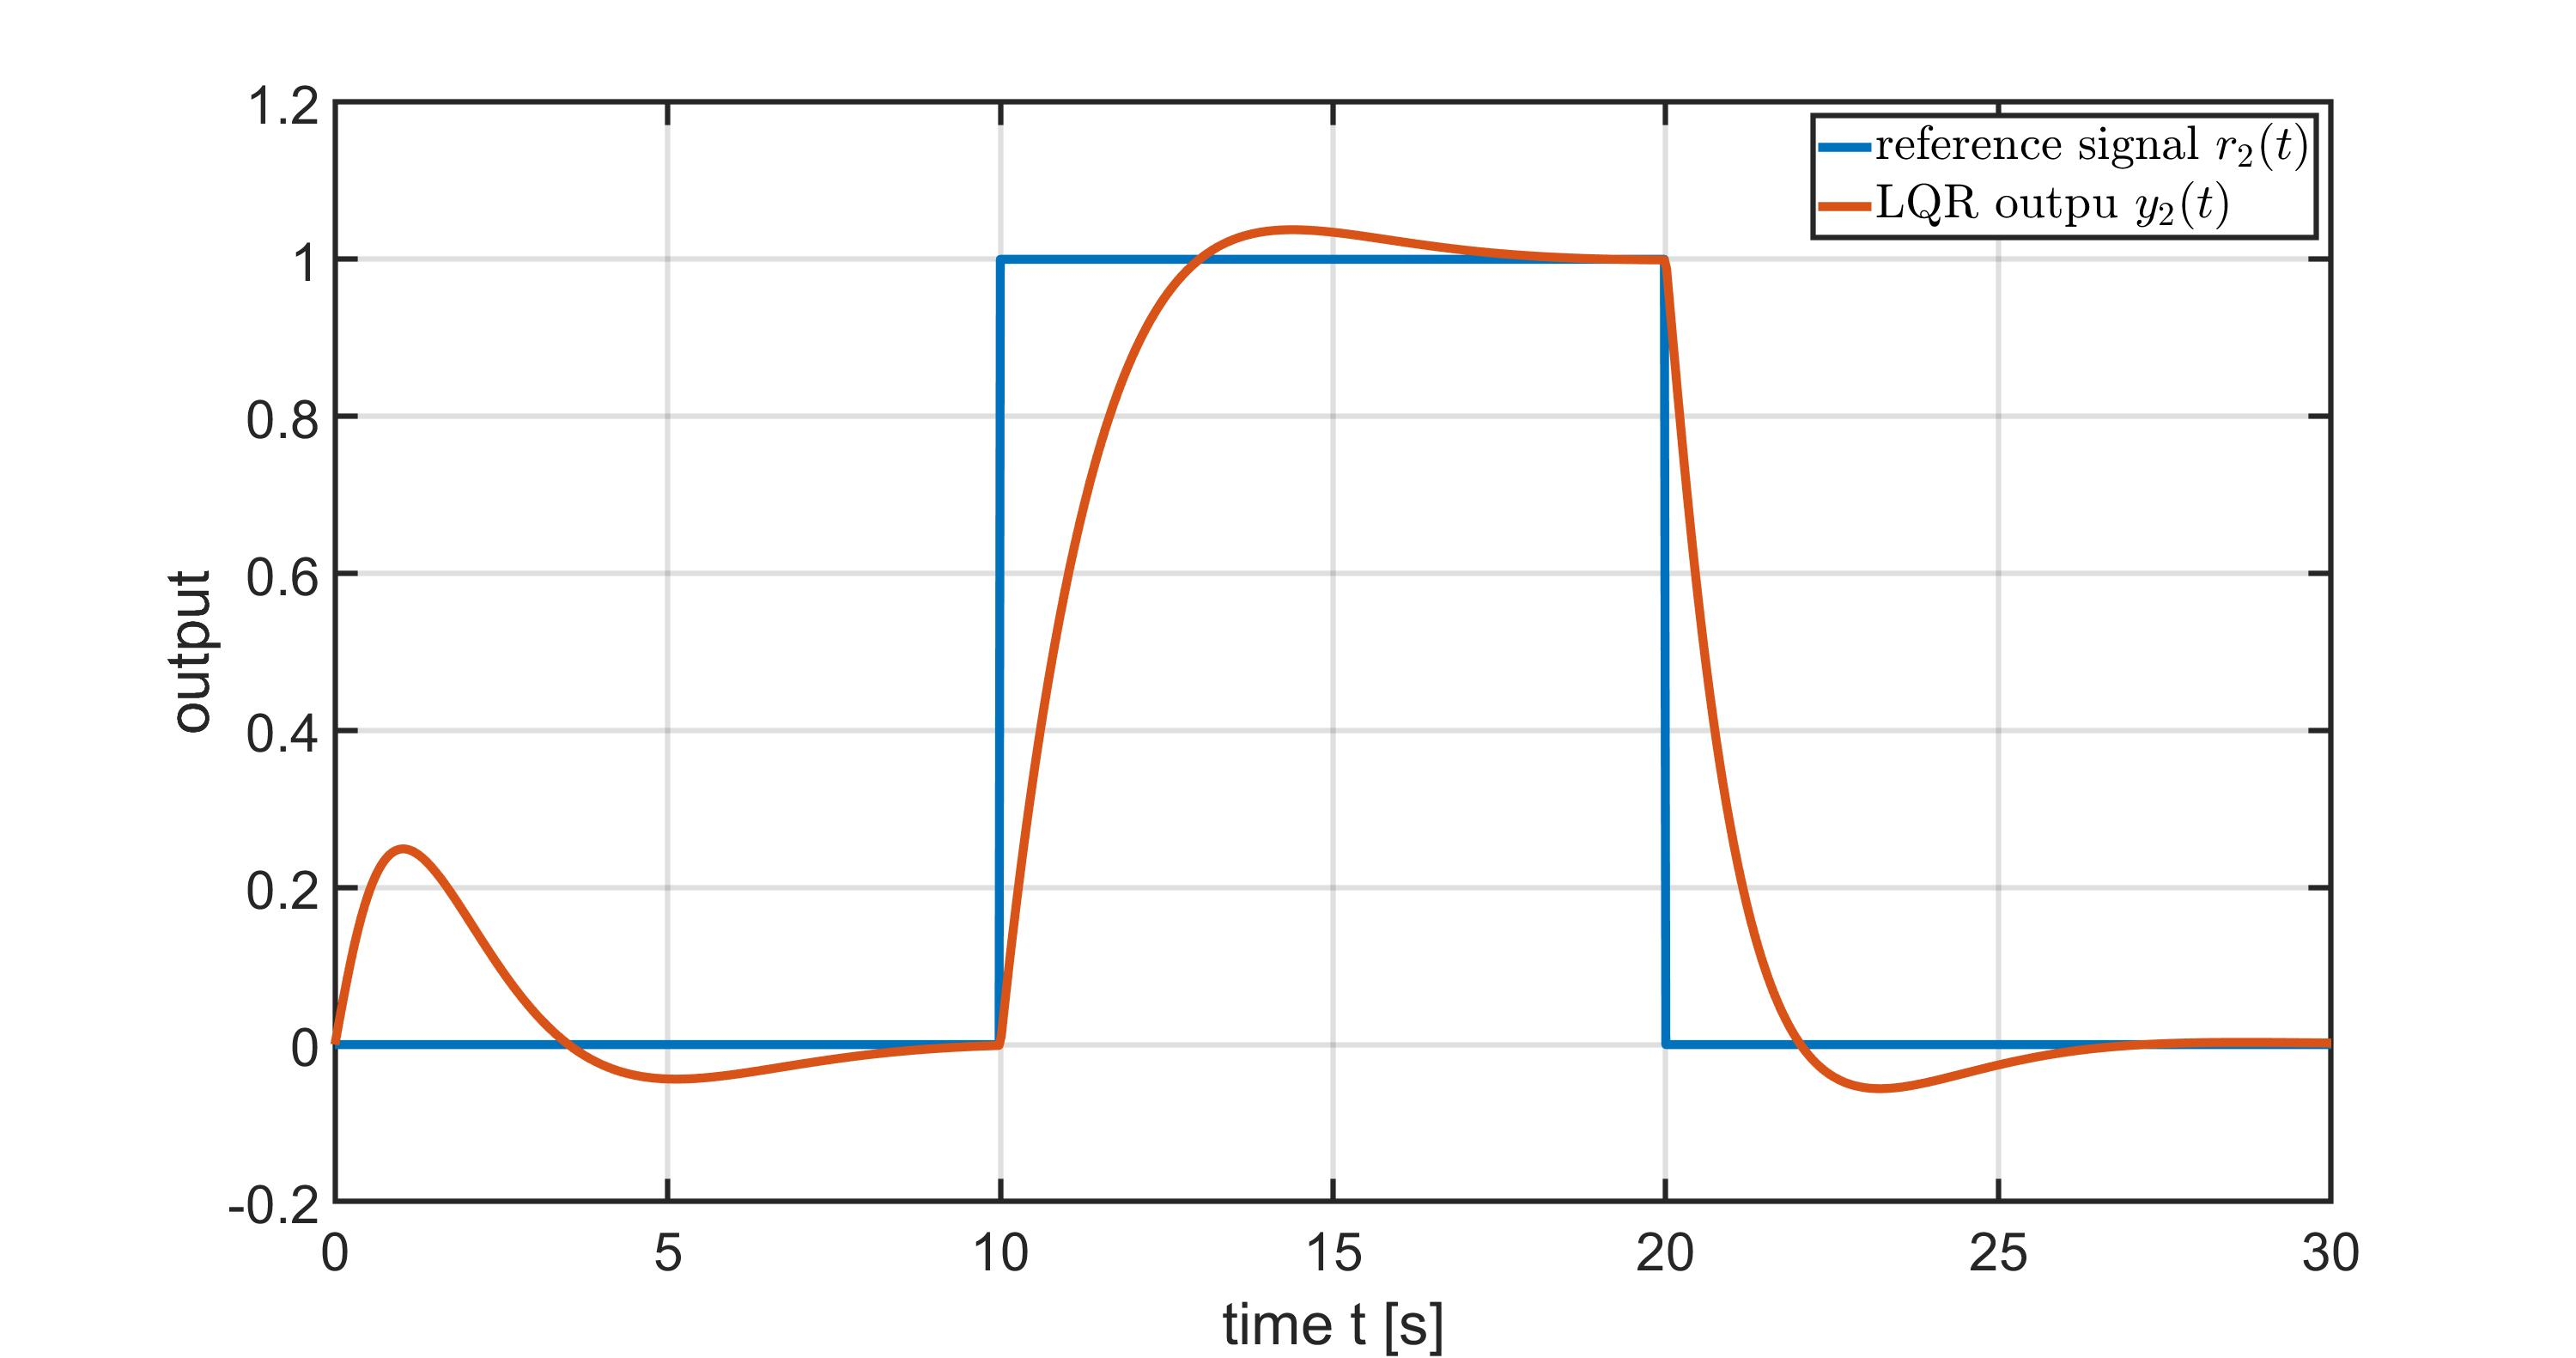
\includegraphics[width=\textwidth]{fig/AC1_LQR_2.jpg}
		\caption{Second signal}
	\end{subfigure}
	\hfill
	\begin{subfigure}[b]{0.3\textwidth}
		\centering
		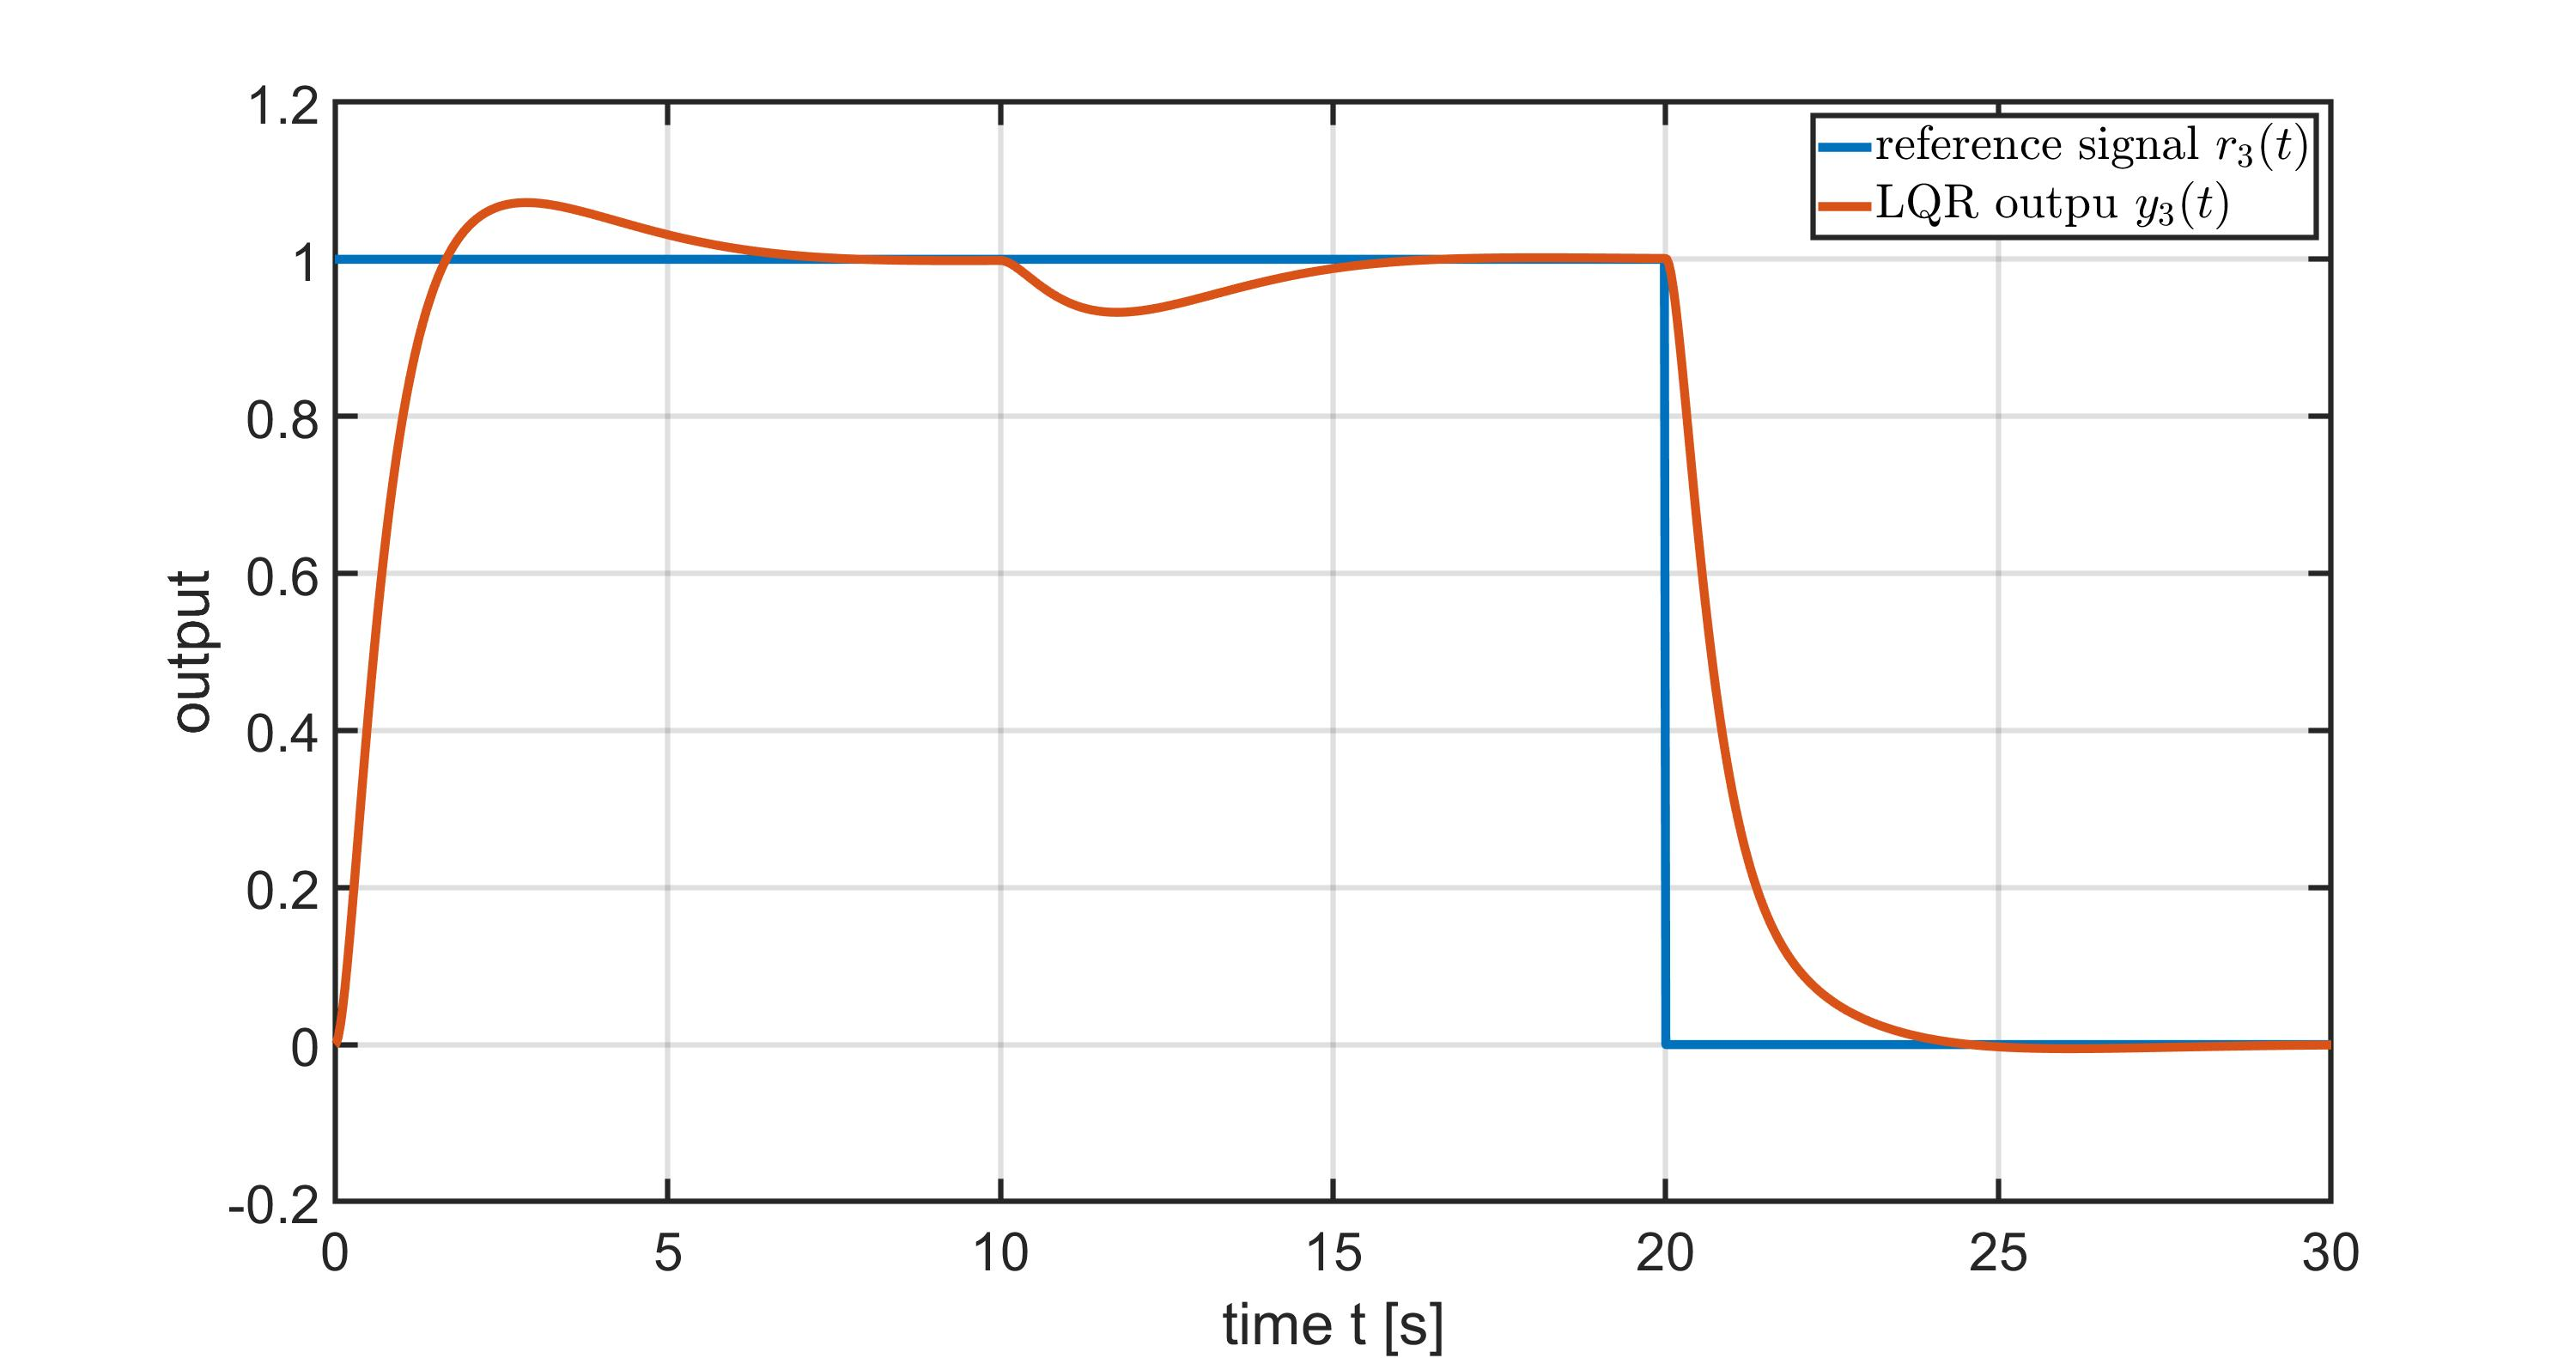
\includegraphics[width=\textwidth]{fig/AC1_LQR_3.jpg}
		\caption{Third signal}
	\end{subfigure}
	\caption{LQR tracking for the system \eqref{eq:Appl:discr_sys}}
	\label{img:Appl:AC1_LQR}
\end{figure}

It looks like something we can improve. However, for $Ts = 10^{-3}$s we get $N = 10^3$ time steps even for one simulation second. The resulting matrix $G$ can not easily be handled and needs vast masses of computer memory. 
\end{exam}

\section{Long time horizon}

	While in originally discrete systems the number of time steps can be not large (as each time step represents one iteration, which does not necessarily depends upon time), the discretezized continuous systems mostly have a large time horizon. 
	
	In Example \ref{ex:ILC:badIA} the Inverse Model Algorithm is not applicable even for $N = 50$. 
	It means, we need a trade off between the time horizon and robustness.
	Already for SISO system the matrix $G$ will have $(N + 1)^2$ elements. 
	
	The more obvious way to reduce the wasted memory is to use the sparse matrices. The matrix $G$ has a lower diagonal structure, what invites to save only the non-zero elements. Even a more space saving method is to save only the last ''line'' of the block matrices 
	\begin{align}
	G_{\rm{line}} = \begin{pmatrix}
	C A^{N-1} B & C A^{N-2} B & \dots & CB D
	\end{pmatrix}.
	\end{align}
	For SDA the matrix $G^\star$ can be perfectly calculated from this simplified form. However, the eigenvalues of the matrix $H$ can not as easily be calculated. However, we can estimate the norm of the matrix $G G^\star$, and choose $\beta$ from a possibly smaller region. 
	
	The solution for PIA  is a bit more complicated. 
	
	
	
	
	
	
	One possibility to reduce the wasted memory is to split our system in the smaller ones. Let us denote the time horizon length with $N_{\max}$, and choose an $N$ with $1<N\leq N_{\max}$
	We can apply our algorithms on the systems with the same state space description, but different initial values. For simplicity, let us assume, that we can divide our time horizon $0,1,2,\dots, N_{\max}$ in $p$ equal parts with time horizon of length $N$\footnote{In a more general case, where $N_{\max}$ can not be devided by $p$ without reminder, We can apply the algorithm one more time on the rest elements, or add them to the last applying iteration of the algorithm.}.  
	
	Then after we  $N$ iterations, we get for the next $N$ iterations the initial condition
	\begin{align}
	x_{0_{\rm{1}}} = A^{N} x(0) + \sum_{\tau = 0}^N A^{\tau}B u(N - \tau). 
	\end{align}
	
	For the next pass we adjust the next initial value as 
	\begin{align}
	x_{0_{\rm{2}}} = A^{2N} x(0) + \sum_{\tau = 0}^{2N} A^{\tau}B u(t - \tau) = A^N x(N+1) + \sum_{\tau = 0}^N A^{\tau} B u(2N - \tau). 
	\end{align}
	
	Doing so fare $1 \leq p^* \leq p$ algorithm passes, we get 
	\begin{align}
	\label{eq:Appl:new_x0}
	\begin{split}
	x_{0_{p^*}} =& A^N x((N+1)(p^* - 1)) + \sum_{\tau = 0}^N A^{\tau}B u(p^*N - \tau) \\
	=&  A^N x_{0_{p^* - 1}} + \sum_{\tau = 0}^N A^{\tau}B u(p^*N - \tau).
	\end{split}	
	\end{align}
	
	That means, we have no need to calculate even more than $N$ powers of $A$. 
	
	However, if the matrix is asymptotically stable, it might have an advantage to neglect some terms $C A^p B$ for $1<p<N$ large enough. 
	It allows us to skip the little elements of the matrix $G$, which might lead to bad condition number. 

	Another benefit of small terms neglecting is the use of sparse matrices. 	
	Our matrix $G$ has a lower triangular structure, and even without any neglecting we can decrease the memory usage by saving only the elements of $G$, which are not zero. With ''reduced'' matrix $G$ we can maintain more space and hence choose a larger $N$ to divide our system in.
	
	The following theorem illustrates it and supposes a method for choosing of this $p^*$. 
	
	\begin{theo}
		\label{thm:Appl:redSys}
	We consider the ''reduced'' lifted system 
	\begin{align}
	\t y = \t G u + d, 
	\end{align}
	\begin{align}
	\t G = \begin{pmatrix}
	D  \\
	CB & D \\
	C A B & CB & D\\
	\vdots & \vdots & \vdots & \ddots \\
	C A^{p^\star-1} B & C A^{p^\star-2}B & C A^{p^\star-3}B &\dots& D \\
	0           & C A^{p^\star-1} B & C A^{p^\star-2} B & \dots & CB & D\\
	0 & 0 & C A^{p^\star-1} B & \dots & CAB & CB & D \\
	\vdots & \vdots & \vdots & \ddots & \vdots & \vdots & \vdots & \ddots \\
	0 & 0 & 0 & \dots & C A^{p^\star-1}& C A^{p^\star-2}B& CA^{p^\star-3}B &\dots & D
	\end{pmatrix}.
	\end{align}
	If $||A||<1$, the error $||y(t) - \t y(t)||$, $p^* < t$, can be estimated undepended on $t$ as 
	\begin{align}
	||y(t) - \t y(t)|| < 2 ||C|| \, ||B|| \,  ||A||^{p^*}\, ||(I - A)^{-1}||\,||u_{\max}||, 
	\end{align}
	with 
	\begin{align}
	||u_{\max}|| = \max_{\tau = 0}^{t - p^*} ||u(\tau)||. 
	\end{align}
	
	$||\cdot||$ denotes here any vector norm and the corresponding induced matrix norm. 

	\end{theo}	
	\begin{proof}
	As $||A||<1$, all the eigenvalues of $A$ are less than 1 in its absolute value and hence the inverse of $(I - A)$ exists. Simple calculation provides 
		\begin{align}
	\begin{split}
			||y(t) - \t y(t)|| &= ||C \sum_{\tau = p^*}^t A^\tau B u(\tau)|| \leq ||C|| \, ||\sum_{\tau = p^*}^t A^\tau || \,||B|| \, ||u_{\max}|| \\
			& = ||C|| \, ||B|| \, ||(A^{p^*} - A^{t + 1})(I - A)^{-1}|| \, ||u_{\max}|| \\
			&  \leq 2 ||C|| \, ||B|| \, ||A||^{p^*} \, ||(I - A)^{-1}|| \, ||u_{\max}||. 
	\end{split}
		\end{align}
	\end{proof}


	This theorem says, that it does not matter how large is our $N$: we still can estimate our output with the same $p^*$. 
	Thou this estimation requires the systems to be asymptotically stable and the norm of the matrix $A$ should be less than one. In addition, this estimation is not very precise, and hence we can not apply this theorem to any system. 
	
	\begin{exam}
		Four our system \eqref{eq:ILC:Sys_ex1} we have for $||u_{\max}||\leq 1.5$ 
		$||y(t) - \t y(t)|| < 3.4033\, 10^{-11}$ for $N = 40$. Hence, we can apply the algorithms for very long time horizon without getting a large error. 
	\end{exam}

\begin{exam}
	\label{ex:Appl:redN}
	For example \eqref{eq:Appl:satellite_sys} we can not easily apply Theorem \ref{thm:Appl:redSys}: for $p^* = 10 \, 000 $ the estimation refers 
	\begin{align}
	||y(t) - \t y(t)|| \leq 0.8879 \text{ for } p^* < t < N,
	\end{align}
	if $||u_{\max}|| \leq 1$.
	
	One can also try to adapt the controller, such that the closed loop matrix $A$ has the eigenvalues of smaller absolute value. However, in our case it does not seem to be a better solution: $H_\infty$ design does not provide a better applicable solution, and pole placement yields the matrix $F$ with very large values. 
	
	But we still can divide our system in the smaller parts and apply the formula \eqref{eq:Appl:new_x0}. 
	
	Choose $N = 100$, and simulate the system dynamics for 30 seconds with time step of $10^{-3}$. 

But before we illustrate the result, let us consider one more issue. 
	
	
\end{exam}

%\section{Online and Offline learning}
%
%In the real problems we often can not have all the information immediately. If we apply the input sequences on the real system, we might have only the results at current time step and the previous ones. 
%
%This is the difference between online and offline learning. In online mode we only have the information from previous iterations. We can not see in the feature and know what results we will get. In opposite, with offline learning we first calculate the new input sequence with an algorithm, and after that send the calculated result into the system and obtain the output. 
%
%In the case of offline learning no more modification are required. We can discretize the system if it is required, split it in the smaller intervals and apply the algorithms. Especially for simulation this might be a good solution, as we can improve the whole sequence at once. 
%
%The online learning requires a bit more effort. Here we apply a chosen ILC algorithm at each time step. This might need more iterations as offline learning, but still the number might rise not too large: since w already applied the algorithm on te previous steps, the new approach should probably need less trials. 
%
%For online learning, the following pseudo code can be used: 
%\begin{lstlisting}
%x0new = x0
%for i = 1 to N 
%	x0new = A x0new + B u(i)
%	unew = ILC(S, x0, i)
%	u(1:i) = unew
%end for
%
%for i = N+1 to Nmax
%	x0 := A x0new + B u(i) 
%	unew = ILC(S, x0, N)
%	u(i-N:i) = unew
%end for
%\end{lstlisting}	
%
%$ILC(S, x0, k)$
% represents here an ILC algorithm over a system $S$, with initial condition $x_0$ and with $k$ -- given time horizon. 
%
%
%\begin{exam}
%	We continue Example \ref{ex:Appl:redN}, and apply the online learning on it. 
%	The result for IA is illustrrated in the figure TODO. 
%\end{exam}
	
	
	
	